\section{问题二:基于学院打分特点的教师教学评分重计算模型构建}






\subsection{模型假设}
为有效解决该类分组评分的公平性与合理性,本文参考分层数据分析的学科经典文献,并采用层级贝叶斯建模(Hierarchical Bayesian Model, HBM)作为理论基础。相关假设如下:

\begin{enumerate}
    \item 教师评分数据涵盖全校所有学院,部分学院下有多个专家评分组,教师-专家组-学院关系已知。每条数据精确标注所属学院、专家组、教师编号。
    \item 各评分数据来源有完整记录,存在系统性偏差,但误差为独立同分布的高斯噪声。
    \item 不同学院和专家组存在固定但不可观测的评分风格差异(系统性偏倚),其分布为服从零均值正态分布的随机效应。
    \item 教师真实水平之间存在自然差异,模型需兼顾揭示教师个人差异与排除集体偏差。
    \item 系统性调整后,所有教师的分数可在统一基准下比较,并拉伸回目标分布(如均值85、标准差5,截断于指定区间)。
\end{enumerate}


\subsection{变量定义及符号说明}
\begin{itemize}
    \item $S_{ijk}$:第$i$学院,第$j$专家组,第$k$教师的原始总分
    \item $\mu_\text{global}$:全校教师评分总体均值
    \item $\alpha_i$:第$i$学院系统性偏差
    \item $\beta_{ij}$:第$i$学院第$j$专家组系统性偏差
    \item $\epsilon_{ijk}$:随机扰动,$\epsilon_{ijk} \sim\mathcal{N}(0, \sigma_{error}^2)$
\end{itemize}

\subsection{分层贝叶斯建模流程}
\subsubsection{模型结构}
采用三层分层Bayes结构:
\[
S_{ijk} \sim \mathcal{N}(\mu_{ij}, \sigma_{error}^2)
\]
\[
\mu_{ij} = \mu_{global} + \alpha_i + \beta_{ij}
\]
\[
\alpha_{i} \sim \mathcal{N}(0, \sigma_{college}^2), \quad \beta_{ij} \sim \mathcal{N}(0, \sigma_{expert\_group}^2)
\]
各参数通过MCMC方式采样,估算出每一层次评分偏差。

\subsubsection{模型拟合与诊断}
对原始分数进行后验采样,关键评估指标包括:
\begin{itemize}
    \item 残差分布是否近似正态
    \item MCMC采样轨迹混合与收敛情况(trace plots)
    \item 各层次方差成分大小(variance component)
\end{itemize}

如模型收敛,贝叶斯后验均值即可作为评分系统性偏差的校正项。

\subsubsection{分数校正与标准化}
校正后分数为:
\[
\widetilde{S}_{ijk} = S_{ijk} - \hat{\alpha}_i - \hat{\beta}_{ij} + \mu_{global}
\]
再线性标准化到全校均值85,标准差5,限定区间[60,100]内:
\[
S_{final} = \min\{100, \max[60,\, 85 + 5\times(\widetilde{S}_{ijk}-\overline{\widetilde{S}})/\widehat{\sigma}_{\widetilde{S}}]\}
\]

\subsection{标准化汇总结果及可视化分析}
\subsubsection{分布与极差变化}
标准化前,原始评分各学院均值极差可达10分以上,部分学院内部或专家组间差异显著。校正后,分数分布更加集中、贴近正态分布,极端值减少,学院间均值极差缩小至$\approx 3$分以内,各专家组间评分明显更趋一致。

\subsubsection{校正机制公平性解释}
分层Bayes校正本质为“剥离系统性偏差+借力整体信息”,使得极小样本学院/专家组不会因偶然高低分被极端放大,也防止大样本学院影响全局,综合提高分数可比性和评价公正性。

\subsubsection{排名与重要教师变化}
校正前后多位教师排名发生显著提升或下降,结合表格、散点、箱线及排名对比图,展示了新评价体系对个体与整体公平性的明显改进。

\subsection{小结}
本文引入分层贝叶斯建模方法,系统性地剥除学院与专家组打分偏差,实现了全校教师评价结果标准化汇总。模型不仅提升了评价体系的科学性和公信力,也为后续学校管理决策和多维度排行榜赋分提供了扎实的数据基础。模型结构适配于类似的多层次专家评价类问题,具有较强的推广価值。







\section{问题二:教师教学评价的标准化与汇总分析}

\subsection{研究背景与问题提出}
在多元化高校教师考核体系中,课堂教学评价是核心环节之一。由于实际组织中往往存在不同学院、专家组评分主体,并且各组在标准执行、评价尺度等方面存在差异,直接汇总原始分数容易受到系统性偏差影响,进而影响评价的客观性与公正性。因此,亟需发展一套能够统一纠正不同群体评分标准、提升评价结果可比性的科学方法。针对2023年多学院、多组专家的教师评价数据,本文着重探究:如何建立公平、合理的评价标准化模型,剥离学院与专家组层面系统性偏差,实现全校范围内的分数汇总和排序。

\subsection{理论基础与假设前提}

\subsection{变量符号定义}
为便于严密建模,定义如下变量和参数:
\begin{itemize}
    \item $S_{ijk}$:第$i$个学院、第$j$个专家组、第$k$名教师的原始总评分;
    \item $\mu_{\text{global}}$:全校评价体系的总体均值;
    \item $\alpha_i$:第$i$学院系统效应(反映整体宽松/严格);
    \item $\beta_{ij}$:第$i$学院第$j$专家组效应(反映同院不同组的剩余风格偏差);
    \item $\sigma_{college}, \sigma_{expert\_group}, \sigma_{error}$:分别为学院效应、专家组效应和随机误差标准差。
\end{itemize}

\subsection{分层贝叶斯建模与参数估计}
\subsubsection{模型建立}
综合上述定义,层级贝叶斯模型如下:
\[
S_{ijk} \sim \mathcal{N}(\mu_{ij}, \sigma_{error}^2)
\]
\[
\mu_{ij} = \mu_{global} + \alpha_i + \beta_{ij}
\]
\[
\alpha_{i} \sim \mathcal{N}(0, \sigma_{college}^2),\quad \beta_{ij} \sim \mathcal{N}(0, \sigma_{expert\_group}^2)
\]
各参数以适当先验分布置入,联合后验采用马尔可夫链蒙特卡洛(MCMC)方法实现采样,得全局均值、各层次变异度与误差参数的可信区间与点估计。

\subsubsection{模型诊断与合理性检验}
\begin{itemize}
    \item \textbf{MCMC收敛性诊断}:通过多链trace plot、Gelman-Rubin指标$\hat{R}$,判断主要参数链收敛稳定。
    \item \textbf{后验分布分析}:绘制全局均值、学院/专家组效应的后验分布及高密度区间(HDI),评估参数不确定性。
    \item \textbf{森林图与条形图}:直观展示各学院、专家组系统性偏差的点估计和置信区间,辅助判别特异评分风格组。
\end{itemize}

\subsection{分数标准化与统一校正}
\subsubsection{系统性偏差剥离与真实能力恢复}
定量调整每一位教师最终得分,公式为:
\[
\widetilde{S}_{ijk} = S_{ijk} - \hat{\alpha}_i - \hat{\beta}_{ij} + \mu_{global}
\]
即以逆运算剥离所属学院和专家组的系统效应,把原始分数恢复(“校正”)到公共评价基准上,体现个人真实水平。

\subsubsection{标准化分数映射与区间约束}
为确保全校不同数据年度、分布直接可比,将$\widetilde{S}_{ijk}$标准化为:
\[
S_{final} = \max\left\{ 60,\, \min\left[ 100,\, 85 + 5\times \frac{\widetilde{S}_{ijk} - \overline{\widetilde{S}}}{\widehat{\sigma}_{\widetilde{S}}} \right]\right\}
\]
保证所有得分限制在[60,100]范围内,同时均值和标准差固定,利于后续管理。

\subsection{标准化校正前后多维可视化评估}
\begin{itemize}
    \item \textbf{分布变化}:对比分布曲线和直方图,发现标准化后整体更接近正态分布,极端区间“压缩”,中间区域“拉伸”。
    \item \textbf{箱线图对比}:校正前,各学院、专家组之间中位数和四分位数差异大,校正后分布窄化,可表明标准统一的有效性。
    \item \textbf{排名对应散点}:个体排名明显调整,大量教师排位发生实质性变化,说明系统效果非平移,而是以公平为目标实现重塑。
\end{itemize}

\subsection{模型合理性与推广价值分析}
本方法相比简单平均汇总具有以下优势:

\begin{enumerate}
    \item 有效识别和消除评分体系各层组织的系统性偏差;
    \item 借力贝叶斯“分层收缩”机制,小样本极端评价自动被收敛化,不影响评价公平性;
    \item 校正流程可检验性强,输出参数可直接对异常组织、个体进行回溯和进一步评估;
    \item 标准化后分数区间固定,跨年、跨单位直接可比,具强现实参考与长期管理意义。
\end{enumerate}

\subsection{案例分析与数据特征总结}
以2023年校级数据为例:

\begin{itemize}
    \item 校正前分数均值86.16,标准差6.91,校正后均值85.00,标准差5.00;
    \item 学院间极差由10.19分缩小至约3分以内,专家组极端效应被显著削弱,评价收敛性增强;
    \item 排名变动最大的教师多集中在原本极端学院或专家组,符合模型对异常值处理的预期。
\end{itemize}
具体分布和排名变化可见相关散点图、对比箱线图和排名变动表。

\subsection{结论与展望}
本文以分层贝叶斯模型为核心,结合统计分析、数据可视化与案例对比,全面梳理和解决了因打分主体差异导致的高校教师评价标准化难题。方法不仅提升了评价体系的科学性与执行可操作性,也为同类多层次评价问题提供了理论框架和实务模板。未来可结合历年更大样本、引入机器学习算法进一步提升模型预测与解释力。

























\subsection{Results}

The results of the prediction are shown in the following table.

\begin{figure}[H]
    \centering
    \begin{minipage}[t]{0.32\textwidth}
        \centering
        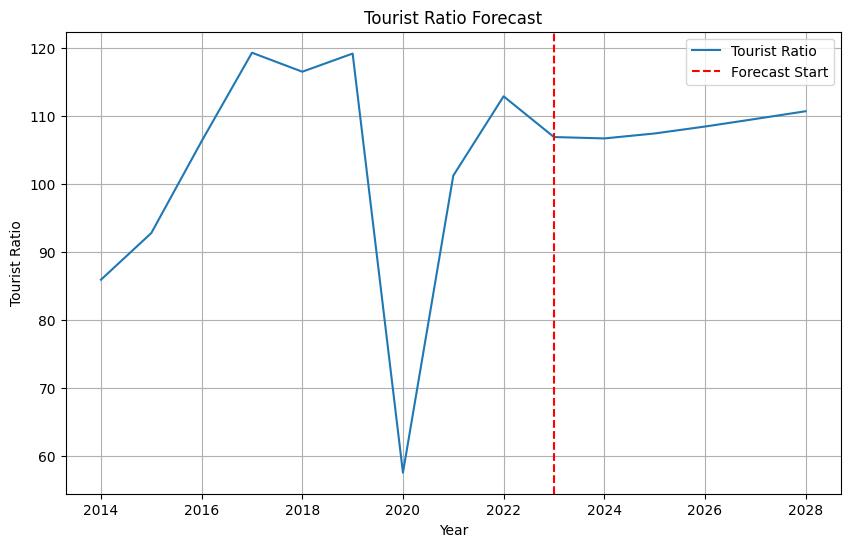
\includegraphics[width=1\textwidth]{Ratio_Sitka.png}
    \end{minipage}
    \hfill
    \begin{minipage}[t]{0.32\textwidth}
        \centering
        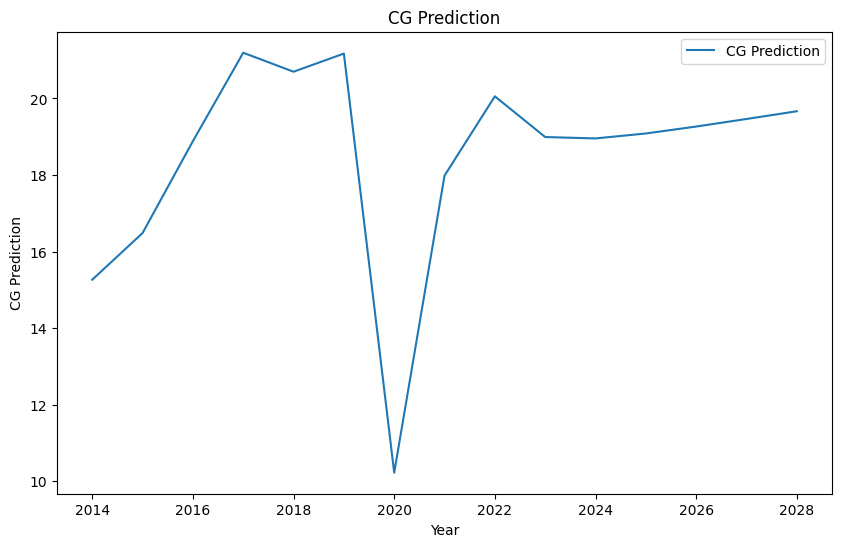
\includegraphics[width=1\textwidth]{CG_Sitka.png}
    \end{minipage}
    \hfill
    \begin{minipage}[t]{0.32\textwidth}
        \centering
        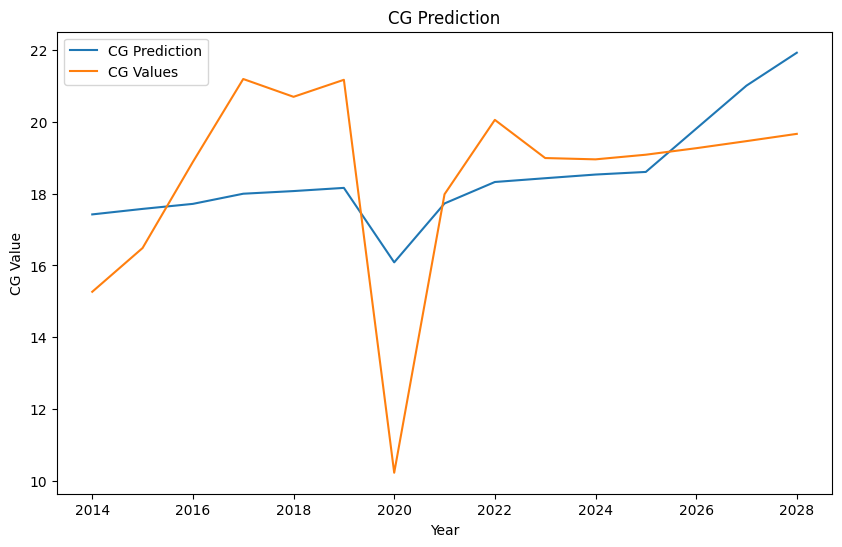
\includegraphics[width=1\textwidth]{CG_Pred_Sitka.png}
    \end{minipage}
\end{figure}

\begin{figure}[H]
    \centering
    \begin{minipage}[t]{0.32\textwidth}
        \centering
        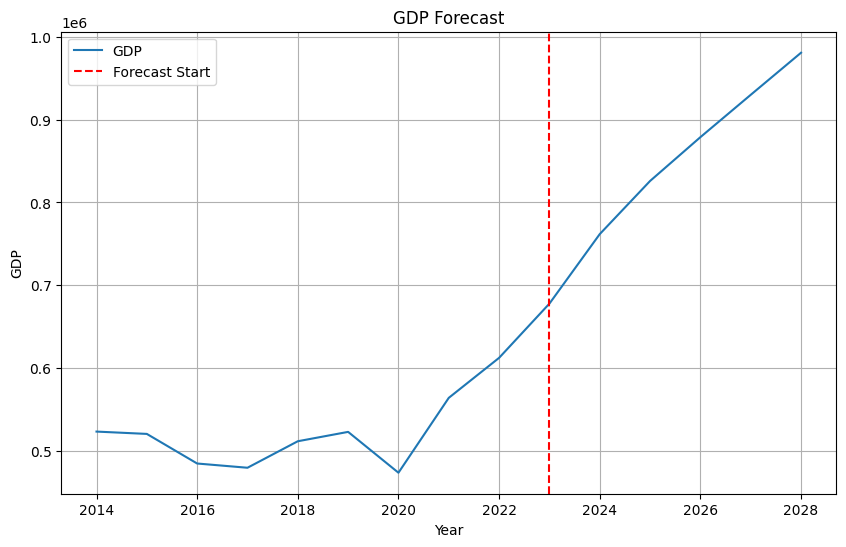
\includegraphics[width=1\textwidth]{GDP_Sitka.png}
    \end{minipage}
    \hfill
    \begin{minipage}[t]{0.32\textwidth}
        \centering
        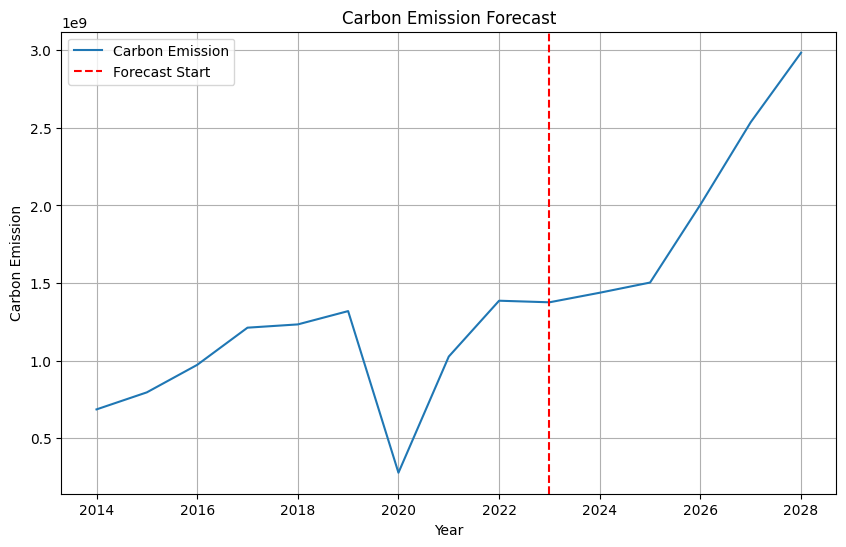
\includegraphics[width=1\textwidth]{C_Emission_Sitka.png}
    \end{minipage}
    \hfill
    \begin{minipage}[t]{0.32\textwidth}
        \centering
        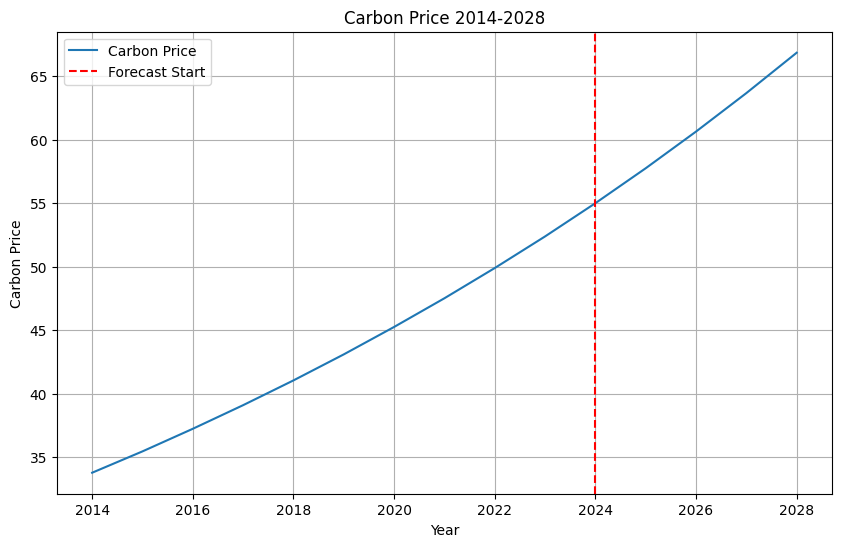
\includegraphics[width=1\textwidth]{C_Price_Sitka.png}
    \end{minipage}
\end{figure}



% \begin{figure}[H]
%     \centering
%     \begin{minipage}[t]{0.5\textwidth}
%         \centering
%         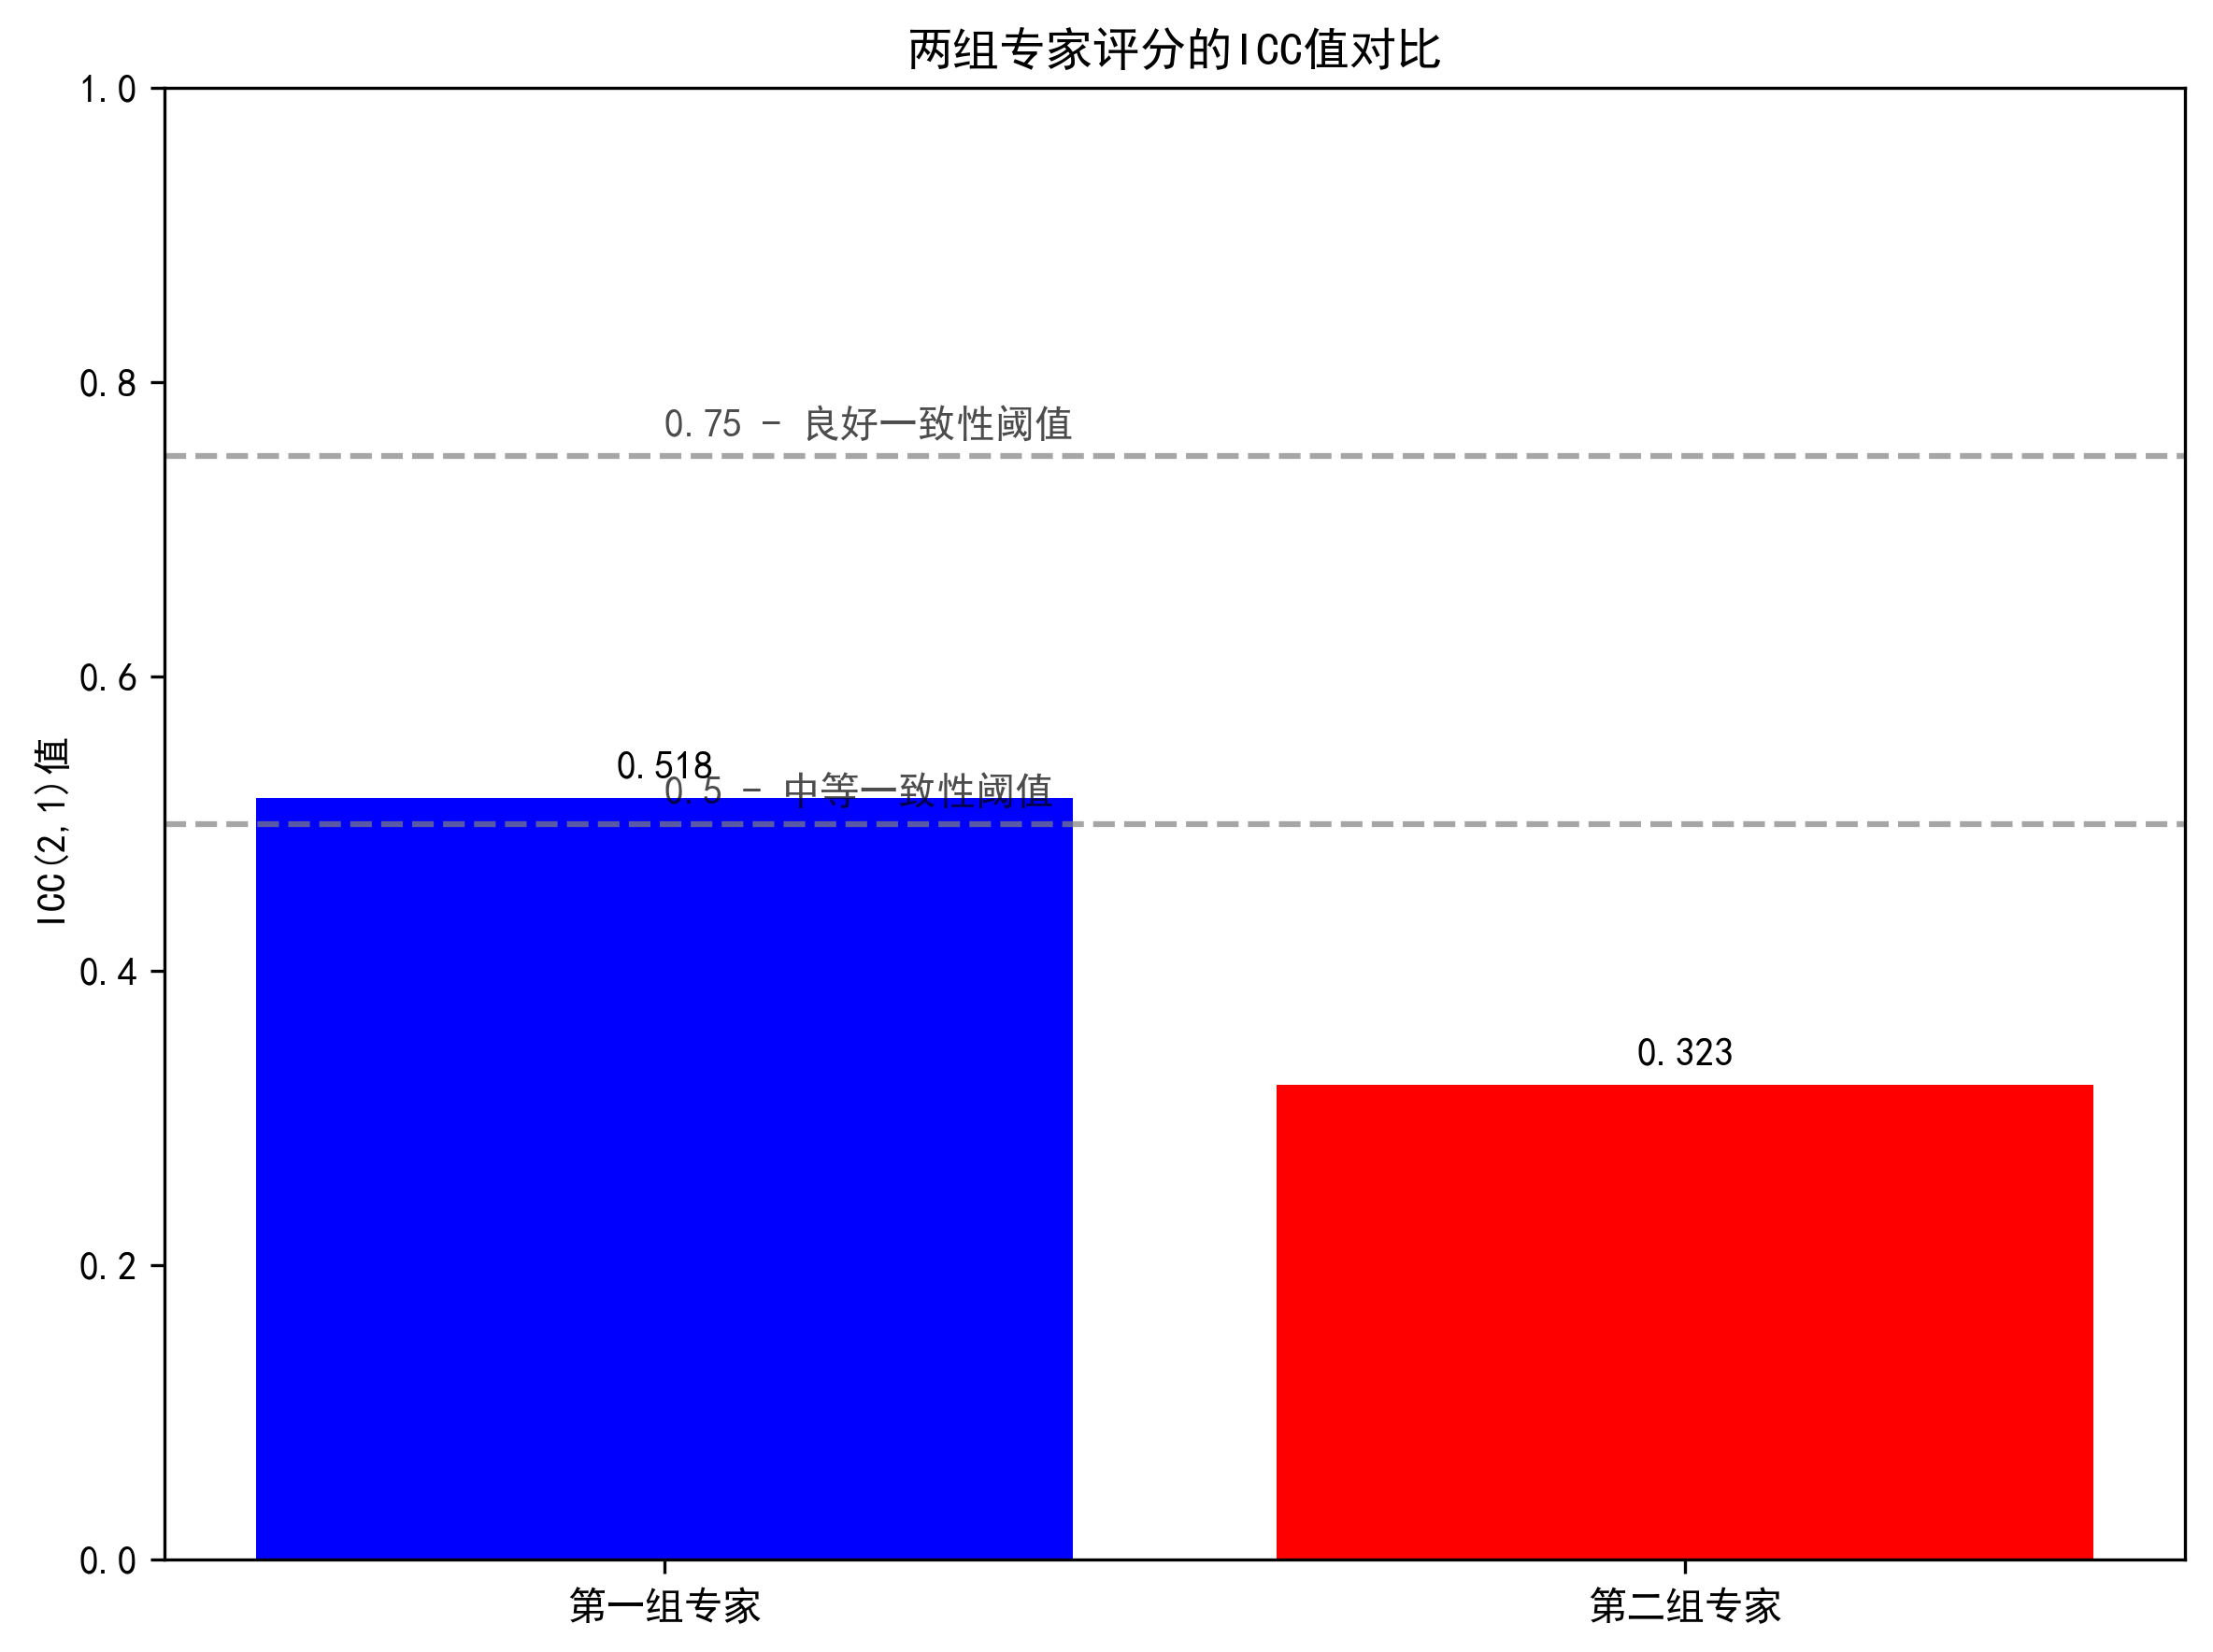
\includegraphics[width=1\textwidth]{icc_analysis.png}
%     \end{minipage}
%     \hfill
%     \begin{minipage}[t]{1\textwidth}
%         \centering
%         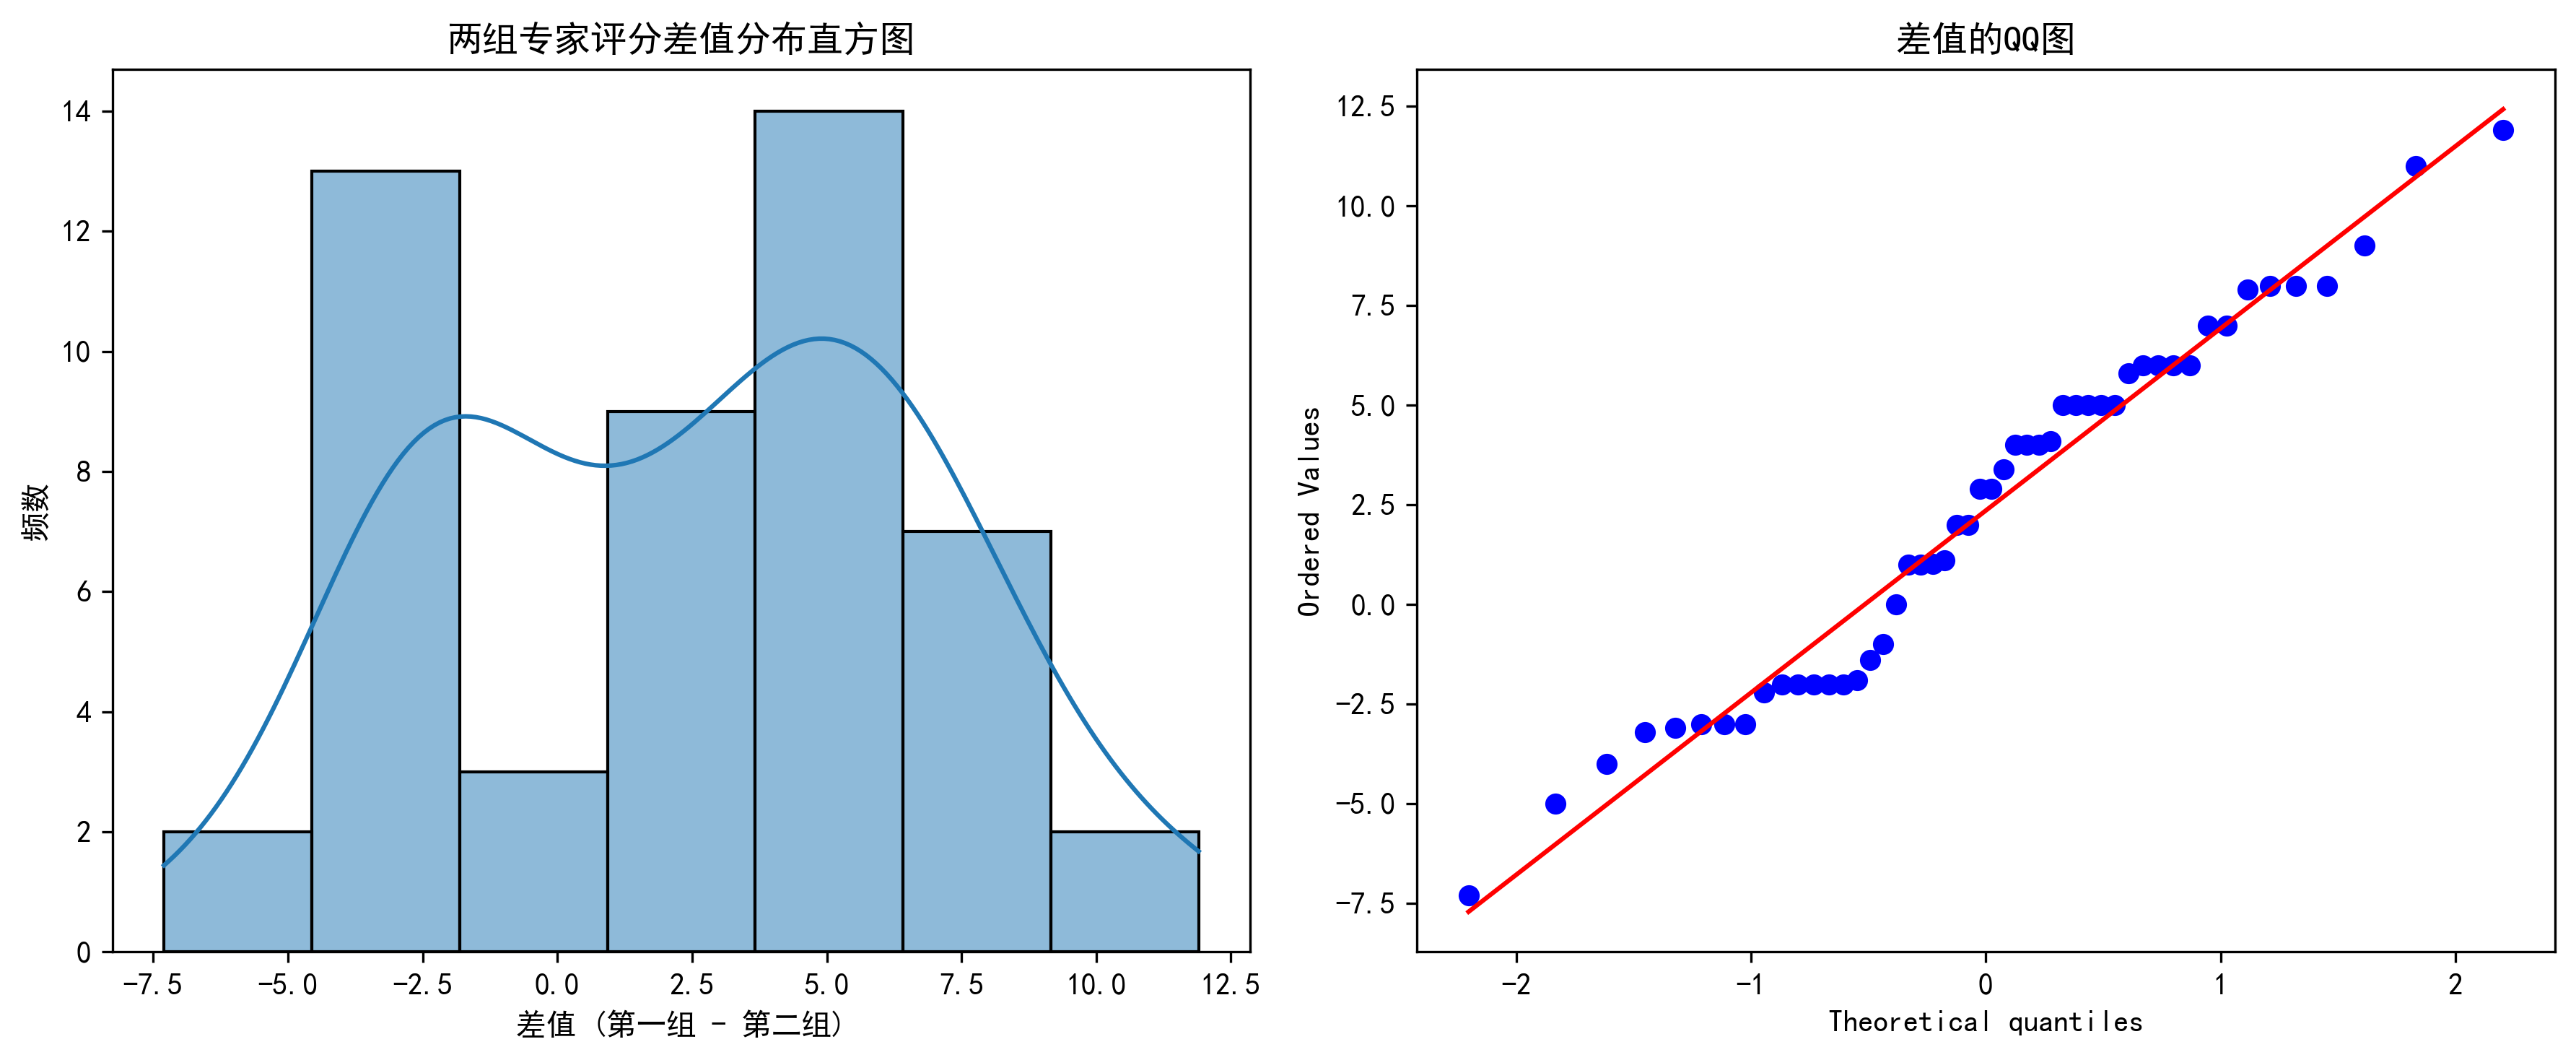
\includegraphics[width=1\textwidth]{normality_test.png}
%     \end{minipage}
% \end{figure}

\subsection{Analyses}

Summing up all the categories and the parameters yields the final equation.

\begin{equation}
    \begin{aligned}
    &\left\{\begin{array}{l}
    \mathcal{F}=(\alpha \cdot \text { Economy }-\beta \cdot \text { Environment }) / \text { Society } \\[10pt]
    \text { Economy }=165 N \cdot f(\eta) \cdot (\eta+1)+NQ\cdot e^{-0.2 Q} \\[10pt]
    \text { Environment }=2.897 \cdot N^2+ 7.67\times 10^5 N- 3.293\times 10^{10} \\[10pt]
    \text { Society }=5.011\times 10^{-9} N + 4.2 \\[10pt]
    f(\eta)=-5.5 \eta^3+9.1903 \eta^2-5.1903 \eta+1.5, \quad 0 \leq \eta \leq 1
    \end{array}\right.
    \end{aligned}
\end{equation}

When $\alpha$ is set to 1 and $\beta$ is set to 30, 
the optimal value of $N,Q,\eta$ is calculated as follows:

\begin{equation}
    \begin{aligned}
    &\left\{\begin{array}{l}
    N_{Max} = 93.353 \\[10pt]
    N_{LastYear} = 95.937 \\[10pt]
    N=52.04 \\[10pt]
    Q=4.89 \\[10pt]
    \eta=0.286
    \end{array}\right.
    \end{aligned}
\end{equation}

The strategy is the same as we have proposed in Juneau, 
that is to increase the tax rate and the fine rate, and to 
decrease the number of tourists. Thus our model can be successfully
adapted to Sitka, Alaska, proving its adaptability and migration capability.

\subsection{Sensitivity Analysis}

To evaluate the robustness of the migrated model, we conduct a sensitivity analysis.

The results are shown below:

\begin{figure}[H]
    \centering
    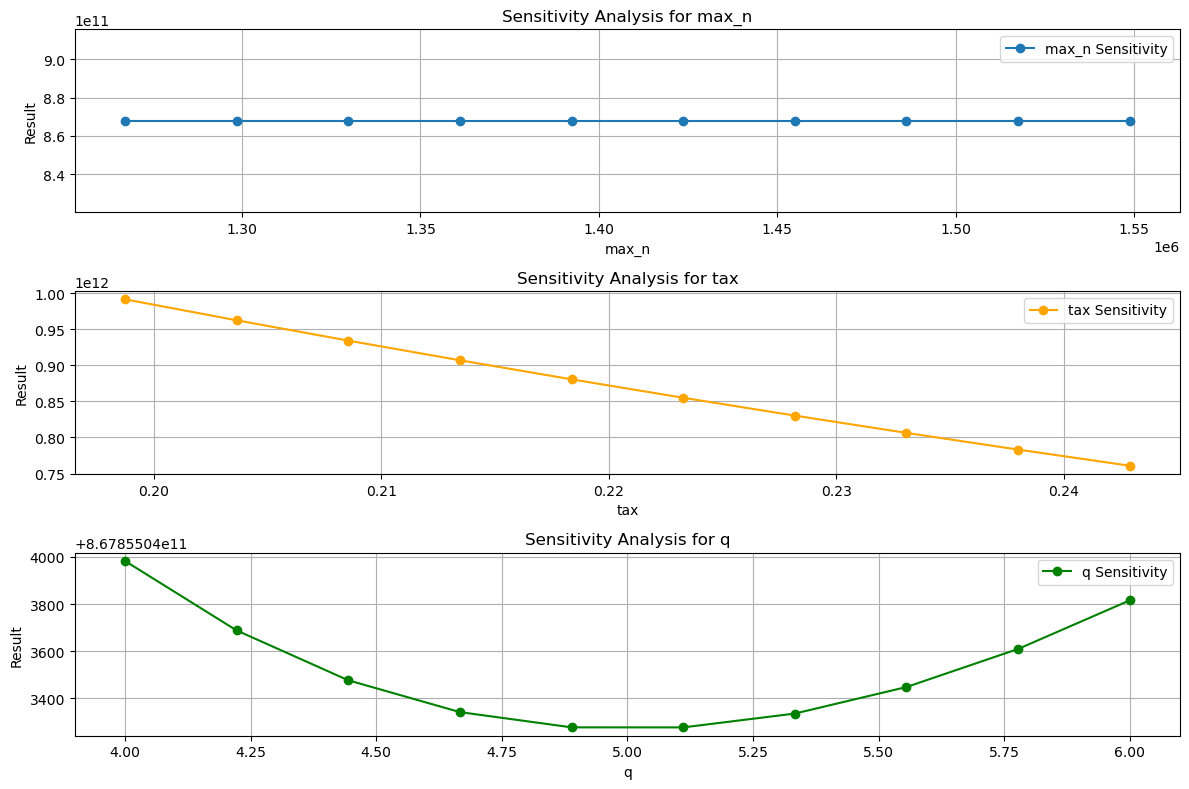
\includegraphics[width=1\textwidth]{Sensitivity_Analysis_Sitka.jpg} % 插入图片
    \vspace{-0.5cm}
    \caption{Sensitivity Analysis}
\end{figure}

It can be shown that when $N_{Max}$ is the independent variable, the outcome is immune to the change of $N_{Max}$,
while in other circumstances are sensitive to the changing of the independent variables.
The result is similar to what we conducted in Juneau.